\section{Recursion and language infinity}

Recursive grammars are essential for generating infinite languages.
\begin{definition}
    A derivation $A\overset{n}{\implies}xAy$ is \emph{recursive} if $n \geq 1$. 

    If $n=1$ the derivation $A\overset{n}{\implies}xAy$ is called \emph{immediately recursive}. 

    The symbol $A$ in the derivation $A\overset{n}{\implies}xAy$ is called \emph{recursive nonterminal}. 

    If $x=\varepsilon$, the derivation $A\overset{n}{\implies}xAy$ is called \emph{left recursive}.

    If $y=\varepsilon$, the derivation $A\overset{n}{\implies}xAy$ is called \emph{right recursive}.
\end{definition}
It's important to note that a grammar can be recursive without being circular.

The necessary and sufficient condition for language $L(G)$ to be infinite is that, assuming $G$ is clean and devoid of circular derivations, $G$ allows for recursive derivations.
\begin{proof}[necessary condition]
    If no recursive derivation was possible, then every derivation would have a limited length, hence $L(G)$ would be finite. 
\end{proof}
\begin{proof}[sufficient condition]
    The derivation $A\overset{n}{\implies}xAy$ implies the derivation $A\overset{+}{\implies}x^mAy^m$ for any $m \geq 1$ with $x,y \in \Sigma^{*}$ not both empty. 
    Furthermore, $G$ clean implies: 
    \begin{itemize}
        \item $S\overset{*}{\implies}uAv$, which means $A$ is reachable from $S$. 
        \item $A\overset{+}{\implies}w$, which means derivation from $A$ terminates successfully. 
    \end{itemize}
    Therefore, there exist nonterminals that generate an infinite language.
\end{proof}
\begin{property}
    A grammar lacks recursive derivations if and only if the graph of the produce relation is acyclic.
\end{property}
\begin{example}
    Consider the following grammar:
    \[
    \begin{cases}
        S \rightarrow aBc \\
        B \rightarrow ab | Ca \\
        C \rightarrow c
    \end{cases}
    \]
    The corresponding graph of the produce relation is shown below:
    \begin{figure}[H]
        \centering
        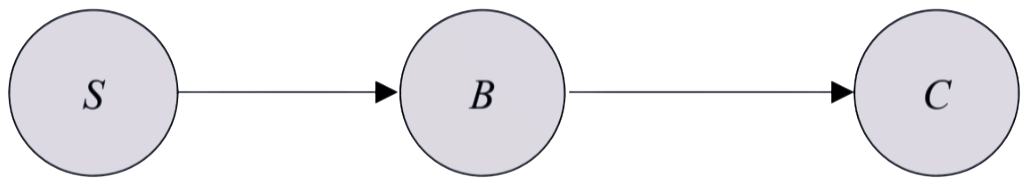
\includegraphics[width=0.5\linewidth]{images/produce.png}
    \end{figure}
    This graph is acyclic, which indicates that the grammar is not recursive.
\end{example}
\newpage